
\title{RECENT DEVELOPMENTS IN HODGE THEORY: A DISCUSSION OF TECHNIQUES AND RESULTS}
\markright{RECENT DEVELOPMENTS IN HODGE THEORY: A DISCUSSION OF TECHNIQUES AND RESULTS}

\author{By~ PHILLIP GRIFFITHS and WILFRIED SCHMID}
\markboth{PHILLIP GRIFFITHS and WILFRIED SCHMID}{RECENT DEVELOPMENTS IN HODGE THEORY: A DISCUSSION OF TECHNIQUES AND RESULTS}

\date{}
\maketitle

%\setcounter{page}{21}
\setcounter{pageoriginal}{20}


\section*{Introduction}\label{art4-sec1}
In\pageoriginale this paper, we shall review several recent developments in \textit{Hodge theory}, as applied to the study of the cohomology of algebraic varieties. In some sense, we are continuing the report \cite{art4-key21} of the first author, in which the then current work in Hodge theory was discussed without proof and a number of open problems were raised. Here we shall be concerned primarily with \textit{methods of proof}, \iec understanding in as transparent terms as possible the techniques utilized in this recent work in Hodge theory. We shall also present some results, due to the second author \cite{art4-key41}, which have just now been published, and shall bring up to date the status of the problems raised in \cite{art4-key21}.

One of the recent developments we shall discuss is Deligne's theory of \textit{mixed Hodge structures} (\cite{art4-key12}, \cite{art4-key}, \cite{art4-key14}). In this work, Deligne extends classical Hodge theory first to open, smooth varieties \cite{art4-key13}, then to complete, singular varieties \cite{art4-key14}, and finally to general varieties, also in \cite{art4-key14}. The heuristic reasoning explaining why such a theory should be possible is given in \cite{art4-key12}.

Deligne's technique is to use \textit{resolution of singularities} \cite{art4-key29}, in order to be able in each case to write the cohomology of the variety in question as being derived from the cohomology of K\"ahler manifolds by homological algebra. Typically this process gives the cohomology of the variety as the abutment of a spectral sequence whose $E_1$ or $E_2$ term is the cohomology of a smooth projective variety. Thus the $E_1$ or $E_2$ term has a \textit{Hodge structure}, and in order for this structure to survive as a Hodge structure on $E_\infty$, inducing the desired mixed Hodge structure on the cohomology of the variety, it is necessary that the spectral sequence degenerates. Following a discussion of the formalism of Hodge structures and mixed Hodge structures in \S 1, we have in \S 2 (a), \S 4, and \S 5 (d)  presented several typical degeneration arguments in as direct a manner as we could.

In \S \ref{art4-sec4} we construct the mixed Hodge structure on the cohomology of the simplest singular complete varieties, namely those having only \textit{normal crossings as singularities}. Here the main reason for the various degeneration theorems can be clearly isolated. The result in \S \ref{art4-sec4} stops far short of proving the existence of a mixed Hodge structure on the cohomology of a general singular variety \cite{art4-key14}. However, it is the method by which one most frequently \textit{calculates} this mixed Hodge structure (cf. \cite{art4-key10}, for instance), once it is known to exits.

In \S \ref{art4-sec5}, we have reproved the main result in the open case \cite{art4-key13} from a more analytic and less homological point of view. Our main idea is, instead of using the customary de Rham complex of $C^\infty$ forms on a compact K\"ahler manifold, to utilize a larger complex containing $L^1$-forms with certain precise types of singularities, and where the \textit{Gysin map} can be given on the form level preserving the Hodge filtration. This complex is discussed in \S\ref{art4-sec2}(b), where it is pointed out that the introduction of singular forms is necessary in order to have such a Gysin map on the form level. Operating inside this complex allows us to see clearly the differentials in the relevant spectral sequence in the open case, and to conclude the degeneracy result from the principle of two types (\S\S\ref{art4-sec5}(d), (e)).

Section 6 is devoted to some applications of Deligne's theory. First in \S \ref{art4-sec6}(a), we give his ``theorem on the fixed part'', which is the main tool in Deligne's study of the moduli of Hodge structures. Then, in \S\ref{art4-sec6}(b), we give a direct proof of an interesting result from \ref{art4-13}, concerning meromorphic differential forms on algebraic verieties; and finally we discuss an application of mixed Hodge structures to \textit{intermediate Jacobians} in \S \ref{art4-sec6}(c).

The second technique which we shall explore in some depth is the use of \textit{hyperbolic complex analysis}, as it applies to variation of Hodge structure. Hyperbolic complex analysis is the study of the influence of \textit{negative curvature} on holomorphic mappings. The classifying spaces for variation of Hodge structure are negatively curved, relative to the holomorphic maps which might arise in algebraic geometry (\cf. \cite{art4-key11}, \cite{art4-key25}, and \S \ref{art4-sec3}(a), (b)), and so it is natural to apply the general philosophy in this case.

Following a discussion of the basic \textit{Ahlfors lemma} and its variants in \S \ref{art4-sec7}(a), we have given Borel's proof of the quasi-unipotence of the \textit{Picard-Lefschetz transformation} in \ref{art4-sec7}(b); this should illustrate in a simple fashion the power of the method.

Perhaps the most penetrating use of the philosophy of hyperbolic complex analysis occurs in the \textit{Nevanlinna theory} \cite{art4-key24}, which affords a general mechanism for analyzing the singularities of a holomorphic mapping. Following a preliminary result from Nevanlinna theory in \S \ref{art4-sec8}(a), we have used this technique to give rather simple, geometric proofs of \textit{Borel's extension theorem} \cite{art4-sec5} in \S \ref{art4-sec8}(b), and of the \textit{Riemann extension theorem for variation of Hodge structure} \cite{art4-key19} in \S \ref{art4-sec8}(c).

A final recent development we shall discuss is the work by the second author \cite{art4-key41} and joint work by him and Clemens \cite{art4-key10}, concerning the asymptotic behavior of the Hodge structures on the cohomology groups of an algebraic variety as it acquires singularities. In \S \ref{art4-sec9}(a), we have used the theorem on \textit{regular singular points} (\S \ref{art4-sec3} (c)), together with the Ahlfors lemma, to give an alternate proof of the first theorem from \cite{art4-sec41}. This result, the \textit{nilpotent} orbit theorem, reduces the case of a general degeneration of Hodge structure to the study of a special king a \textit{nilpotent orbit} in a classifying space for variation of Hodge structure. It seems possible to use Nevanlinna theory in place of the theorem on regular singular points to prove the same result, but we have not purshed this here.

The second main theorem from \cite{art4-key41}, the $SL_2$-\textit{orbit theorem}, gives a detailed and somewhat technical description of the nilpotent orbits which can come up when a one-parameter family of Hodge structures degenerates. The proof depends heavily on Lie theory. In \S \ref{art4-sec9}(b), besides stating the theorem, we describe the observations which originally led to the proof, as well as to the statement, of the theorem.

Some applications of these two theorems will be mentioned in \S\ref{art4-sec10}; we also summarize joint results of Clements and the second author about the topology of a degenerating family of projective manifolds, which again are partly based on the two theorems.

We conclude with an appendix, reviewing the current status of the problems and conjectures contained in the report \cite{art4-sec21} of the first author.

\section{Basic definitions}\label{art4-sec1}
(a)~ \textit{Hodge structures.} Let $H_{\bR}$ be a finite dimensional real vector space, containing a lattice $H_{\bZ}$, and let $H=H_{\bR} \otimes_{\bR} \bC$ be its complexification.

\begin{definition}\label{art4-def1.1}
`A Hodge structure of weight $m$' on $H$ consists of a direct sum decomposition
$$
H = \bigotimes_{p+q=m} H^{p,q}, \text{ with } H^{q,p} = \bar{H}^{p,q}
$$
\end{definition}

(Barring denotes complex conjugation.)

\begin{remark*}
The prototypical example is the decomposition according to Hodge type of the $m$-th complex cohomology group of a compact K\"ahler manifold. In this case, $m$, $p$, $q \;\geqslant 0$; however, it will be convenient to admit also negative values for $m$, $p$, and $q$. For example, the \textit{Hodge structure of Tate} $T$(1) is defined by
$$
H_{\bZ} =\bZ, \; H_{\bR} = \bR, \; H = \bC, \; m= -2, \text{ and } H = H^{-1,-1}.
$$

For any two Hodge structures $H, H'$, both of weight $m$, the direct sum $H\oplus H'$ carries an obvious Hodge structure, also of weight $m$. Similarly, if $H$ and $H'$ have possibly different weight $m$ and $m'$,
$$
H\otimes H', \; \Hom (H, H'), \Lambda^p H, \; H^\ast
$$
inherit Hodge structures of weight $m+ m'$, $m'-m$, $pm$, and $-m$, respectively: $\lambda \in \Hom(H, H')$ has Hodge type $(p,q)$ if $\lambda(H^{r,s}) \subset (H')^{p+r, \; q+s}$ for all $r, s$; in particular, this definition applies to $H^\ast = \Hom (H, \bC)$, with $\bC$ carrying the trivial Hodge structure of weight $0; H \otimes H'$ can be identified with $\Hom (H^\ast, H')$, and $\otimes^pH$ induces a Hodge structure on its subspace $\Lambda^p H$.
 \end{remark*}

\begin{definition}\label{art4-def1.2}
A linear map $\varphi: H \to H'$ between vector spaces with Hodge structures will be called a morphism (of Hodge structures) if it is defined over $\bQ$, relative to the lattices $H_{\bZ}$, $H'_{\bZ}$, and if $\varphi (H^{p,q}) \subset (H')^{p,q}$, for all $p,q$. More generally, $\varphi$ is a morphism of type $(r,r)$ if again it is defined over $\bQ$, and if it has type ($r, r$) when viewed as an element of $\Hom(H, H')$.
\end{definition}

As a trivial, but nevertheless important, observation we note that morphism of type $(r,r)$ must vanish unless the weights $m$ and $m'$ of $H$ and $H'$ satisfy $m'=m+2r$.

To\pageoriginale each Hodge structure $H = \oplus_{p+q =m} H^{p,q}$ of weight $m$ one associates the \textit{Hodge filtration}
\setcounter{equation}{2}
\begin{equation}
H \supset \ldots \subset F^{p-1} \supset F^p \subset F^{p+1} \supset \ldots \supset 0 \text{ with } F^p = \oplus_{i \geqslant p} H^{i, m-i}.  \label{art4-eq1.3}
\end{equation}

It may be convenient to visualize the definition by means of the picture below:
\begin{figure}[H]
\centering
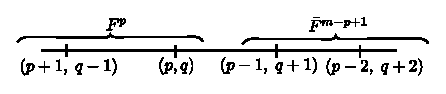
\includegraphics{art4-fig1.eps}
\end{figure}

The Hodge filtration determines the Hodge structure completely, since
\begin{equation}
H^{p,q} = F^p \cap \bar{F}^q \label{art4-eq1.4}
\end{equation}

Conversely, a descending filtration $\{F^p\}$ of $H$ arises as the Hodge filtration of some Hodge structure of weight $m$ if and only if
\begin{equation}
F^p \oplus \bar{F}^{m-p+1} \xrightarrow{\approx} H, \;\; \text{ for all } p.
\label{art4-eq1.5}
\end{equation}

Thus one has a 1:1 correspondence between Hodge structures and Hodge filtrations, \iec filtrations satisfying \eqref{art4-eq1.5}.

In terms of this latter description, a linear map $\varphi: H \to H'$, which shall be defined over $\bQ$, becomes a morphism of type $(r, r)$ exactly when it preserves the Hodge filtration, with a shift by $r$; in other words, when 
\begin{equation}
\varphi (F^p) \subset F'^{p+r}, \;\text{ for all }p. \label{art4-eq1.6}
\end{equation}

Now let $\varphi$ be a morphism of type $(r, r)$, $v$ a vector in $F'^{p+r} \cap \Iim \varphi$. By decomposing a vector in the inverse image of $v$ according to Hodge type, one finds that $v$ lies in the image of $F^p$. Thus:

a morphism of Hodge structures of type $(r,r)$ preserves the Hodge filtrations strictly, with a shift by $r$, in the sense that 
\begin{equation}
\varphi(F^p) = F'^{p+r} \cap \Iim \varphi, \text{ for all } p. 
\label{art4-eq1.7}
\end{equation}

We consider a Hodge structure $H = \oplus_{p+q = m} H^{p,q}$ and a bilinear form $Q$ on $H$, which shall be defined over $\bQ$. Also $Q$ shall be symmetric if $m$ is even, skew if $m$ is odd.

\setcounter{definition}{7}
\begin{definition}\label{art4-def1.8}
The Hodge structure is polarized by $Q$ if 
$$
\begin{matrix}
Q (H^{p,q} , H^{p', q'} =0) & \text{ unless } p = q', \; q = p',\\[2pt]
(\sqrt{-1})^{p-q} Q (v, \bar{v}) > 0 & \text{ for } v \in H^{p,q}, \; v \neq 0.
\end{matrix}
$$
\end{definition}

Apparently, the polarization form $Q$ must be nondegenerate. The Weil operator $C: H \to H$ of the Hodge structure is defined by 
\setcounter{equation}{8}
\begin{equation}
C_v = (\sqrt{-1})^{p-q} v, \text{ for } v \in H^{p,q} . \label{art4-eq1.9}
\end{equation}
In terms of the Hodge filtration and the Weil operator, the two conditions in \ref{art4-def1.8} become equivalent to 
\begin{equation}
\left.
\begin{matrix}
Q (F^p, F^{m-p+1}) = 0\\
Q (C v, \bar{v}) >0 \;\text{  for } v \neq 0.
\end{matrix}\right\}
\label{art4-eq1.10}
\end{equation}

The example we have in mind is the Hodge bilinear form on the primitive part of the cohomology of a smooth, projective variety over $\bC$, as will be discussed below.

It should be mentioned that the operations of tensor product, Hom exterior product, and duality can also be performed in the context of polarized Hodge structures. For example, if $Q$ and $Q'$ are polarization forms for Hodge structures $H$ and $H'$, then the induced bilinear form on $H \otimes H'$ polarizes the product Hodge structure.

\medskip
\noindent
(b)~ \textit{Mixed Hodge structures.} The symbols $H$, $H_{\bR}$, $H_{\bZ}$ shall have the same meaning as in the previous section.

\begin{definition}\label{art4-def1.11}
`A mixed Hodge structure' on $H$ consists of two filtrations,
$$
0 \subset \ldots \subset W_{m-1} \subset W_m \subset W_{m+1} \subset \ldots \subset H,
$$
the `weight filtration' which shall be defined over $\bQ$, and 
$$
H \supset \ldots \supset F^{p-1} \supset F^p \supset F^{p+1} \supset \ldots \supset 0,
$$
the `Hodge filtration', such that the filtration induced by the latter on $Gr_m(W_\ast) = W_m/W_{m-1}$ defines a Hodge structure of weight $m$, for each $m$ (the induced filtration on $Gr_m(W_\ast)$ is given by
$$
F^p (Gr_m (W_\ast)) = W_m \cap F^p/W_{m-1} \cap F^p).
$$
\end{definition}


\begin{remark*}
The notion\pageoriginale of a mixed Hodge structure contains that of a Hodge structure of weight $m$ as a special case; as Hodge filtration one takes the Hodge filtration in the old sense, and the weight filtration is defined by $W_m = H$, $W_{m-1} = 0$.
\end{remark*}

According to the definition of a mixed Hodge structure, only the successive quotients of the weight filtration have direct sum decompositions according to Hodge type. However, the following lemma of Deligne \cite{art4-key13} provides a more subtle global decomposition of $H$. For any pair of integers $(p,q)$, we consider the subspace
\begin{multline*}
I^{p,q} = (F^p \cap W_{p+q}) \cap (\bar{F}^q \cap W_{p+q} + \bar{F}^{q-1} \cap W_{p+q-2} +\\
 + \bar{F}^{q-2} \cap W_{p+q-3} + \ldots).
\end{multline*}
It is certainly not the case that $I^{p,q} = I^{q,p}$, but one does have the congruence $I^{p,q} \equiv I^{q,p} \mod W_{p+q-2}$, as will follow from the proof of lemma \ref{art4-lem1.12} below. This congruence $I^{p,q} \equiv \bar{I^{q,p}} \mod  W_{p+q-2}$ explains why every mixed Hodge structure with a weight filtration of length two splits over $\bR$, into a sum of two Hodge structures of pure weight. This splitting, of course, may be incompatible with the rational structure. As soon as the weight filtration has length greater than two, a ``general'' mixed Hodge structure will not split over $\bR$.

\setcounter{lemma}{11}
\begin{lemma}[\cf. Lemma 1.2.8 of \cite{art4-key13}.]\label{art4-lem1.12}
Under the projection $W_m \to Gr_m (W_\ast), \; I^{p,q}$, with $p+q=m$, maps isomorphically onto the Hodge subspace $Gr_m (W_\ast)^{p,q}$. Moreover,
$$
W_m = \oplus_{p+q\leqslant m} I^{p,q},
$$
and 
$$
F^p = \oplus_{i \geqslant p} \oplus_q I^{p,q}.
$$
\end{lemma}

\begin{proof}
In view of \eqref{art4-eq1.5}, the definition of a mixed Hodge structure amounts to the following:
\begin{align*}
& \text{given any $v \in W_n$ and integers $p,q$, with $p+q=m+1$,}\\
& \text{one can write $v = v'+\bar{v}'' + u $, such that $v' \in F^p \cap W_m$,}\\
& \text{$v'' \in F^q \cap W_m$, and $u\in W_{m-1}$; this decomposition is unique}\\
& \text{modulo $W_{m-1}$}. \tag{$\ast$}\label{art4-eq*}
\end{align*}

In order to prove the first assertion of the lemma, we fix $m$, $p$, $q$, subject to $m=p+q$, and $\alpha \in Gr_m (W_\ast)^{p,q}$. Then $\alpha$ can be represented by some\pageoriginale $v_0\in F^p \cap W_m$, and also by some $\bar{u}_0 \in \bar{F}^q \cap W_m$. Both are unique upto $W_{m-1}$, and $v_0 = \bar{u}_0 + w_0$, for some $w_0 \in W_{m-1}$. By induction on $k$, starting with $k=0$, we shall find vectors
\begin{gather*}
v_k \in F^p \cap W_m, \qquad w_k \in W_{m-1-k}\\
u_k \in F^q \cap W_m + F^{q-1} \cap W_{m-2} + F^{q-2} \cap W_{m-3} + \ldots + F^{q+1-k} \cap W_{m-k}
\end{gather*}
which will be unique up to $W_{m-k}$, such that $v_k$ represents $\alpha$, and $v_k = \bar{u}_k + w_k$. For $k=0$, this has been done $(F^{q+1} \subset F^q !)$.  If $v_k$, $u_k$, $w_k$ have been picked, we apply \eqref{art4-eq*} to $w_k$: we write $w_k = w'_k + \bar{w}''_k + w_{k+1}$, with $w'_k \in F^p \cap W_{m-1-k}$, $w_k \in F^{p-k} \cap W_{m-1-k}$, $w_{k+1} \in W_{m-2-k}$, uniquely modulo $W_{m-2-k}$. The vectors $w_{k+1}, \; v_{k+1} = v_k - w'_k$, $u_{k+1} =  u_k + w''_k$ then have the desired properties. For large enough $k$, $W_{m-1-k} = 0$; hence $\alpha$ has a unique representative in $I^{p,q}$. We may deduce that
$$
W_m = W_{m-1} \oplus (\oplus_{p+q=m} I^{p,q}),
$$
and thus $W_m = \oplus_{p+q\leqslant m} I^{p,q}$. As for the last statement of the lemma, the sum of the $I^{p,q}$ is now known to be direct. Also, one containment is obvious. We consider some $v \in F^p$, and we let $m$ be the least integer for which $v \in W_m$. The image of $v$ in $Gr_m (W_\ast)$ has Hodge components of type $(i, m-i)$, with $i \geqslant p$, because $v \in F^p \cap W_m$. Subtraction off components in the spaces $I^{i,m-i}$, with $i \geqslant p$, we can push $v$ into $W_{m-1}$. Continuing with descending induction on $m$, we find that $v \in \oplus_{i \geqslant p} \oplus \oplus_q I^{i,q}$, as was to be shown.
 
A \textit{morphism} between two mixed Hodge structures $\{H, W_m, F^p\}$,\break $\{H', W'_m, F'^p\}$ is a rationally defined linear $\map \varphi; H \to H'$, such that $\varphi(W_m) \subset W'_m$ and $\varphi (F^p) \subset F'^p$. More generally, a rationally defined linear $map \varphi : H \to H'$ will be called a morphism of mixed Hodge structures of type $(r,r)$ if $\varphi (W_m) \subset W'_{m+2r}$, $\varphi (F^p) \subset F'^{p+r}$, for all $p$ and $m$. In this case, the induced mapping
$$
\varphi: Gr_m (W_\ast) \to Gr_{m+2r} (W'_\ast)
$$
becomes a morphism of type $(r,r)$ relative to the two Hodge structures of weights $m$ and $m+ 2r$, respectively.
\end{proof}

\setcounter{lemma}{12}
\begin{lemma}\label{art4-lem1.13}
A morphism\pageoriginale of type $(r,r)$ between mixed Hodge structures is strict with respect to both the weight and Hodge filtrations, with the appropriate shift in indices. More precisely, $\varphi (W_m) = W'_{m+2r} \cap \Iim \varphi, \; \varphi (F^p) = F'^{p+r} \cap \Iim \varphi$.
\end{lemma}

\begin{proof}
The definition of the subspaces $I^{p,q}$ immediately gives the containments $\varphi(I^{p,q}) \subset I'^{p+r, q+r}$. Now let $v \in W'_{m+2r} \cap \Iim \varphi$, so that $v = \varphi (u)$ for some $u \in H$. According to \ref{art4-lem1.12},
$$
u = \sum_{p,q} u^{p,q}, \text{ with } u^{p,q} \in I^{p,q}.
$$
Then $\varphi (u^{p,q}) \in I'^{p+r , q+r}$, and $v =\sum_{p,q} \varphi (u^{p,q}) =in W'_{m+2r}$. Again appealing to \ref{art4-lem1.12}, we deduce that $\varphi(u^{p,q}) =0$, unless $p+q \leqslant m$. Hence
$$
v = \varphi \left(\sum_{p+q \leq m} u^{p,q} \right) \in \varphi (W_m).
$$

The case of the Hodge filtration is treated similarly.
\end{proof}

\begin{lemma}\label{art4-lem1.14}
Let $\varphi: H \to H'$ be a morphism of mixed Hodge structures of type $(r,r)$. Then the induced Hodge and weight filtrations put mixed Hodge structure both on the kernel and the cokernel.
\end{lemma}

\begin{proof}
As for the kernel, given $v \in \ker \varphi \cap W_m$ and any integer $p$, we must exhibit vectors
$$
v'\in \ker \vaphi \cap W_m \cap F^p, \; v'' \in \ker \varphi \cap W_m \cap F^{m-p+1}, \; w \in \ker \varphi \cap W_{m-1},
$$
such that $v = v' + \bar{v}''+u$, and these must be uniquely determined modulo $\ker \varphi \cap W_{m-1}$. The uniqueness already follows from the corresponding statement about $H$. Also, there do exist $u'\in W_m \cap F^p$, $u'' \in W_m \cap F^{n-p+1}$, such that $v \equiv u' + \bar{u}'' \mod W_{m-1}$. Since $\varphi(v) = 0$, we conclude that $\varphi (u')$, $\varphi (u'') \in W'_{m+2r-1}$. By appealing to \ref{art4-lem1.12} and decomposing $u'$ into its components in the subspaces $I^{s,t} \subset H$, we can find $u'_1 \in W_{m-1} \cap F^p$, so that  $\varphi(u') = \varphi(u'_1)$. Similarly, $\varphi (u'') = \varphi (u''_1)$ for some $u''_1 \in W_{m-1} \cap F^{m-p+1}$. The vectors $v'= u'-u'_1$, $v''=u'' - u''_1$, $w = v - v'-\bar{v}''$ have the desired properties. In order to prove the assertion about the cokernel, one only has to check one nontrivial fact: if $u \in W'_m \cap F'^p$, $v \in W'_m \cap F'^{m-p+1}$, and if $u + \bar{v} \in w'_{m-1} +\Iim \varphi$, then $u, v\in W'_{m-1} + \Iim \varphi$. Using \ref{art4-lem1.12}, this can be done, in a manner similar to the argument above. Details are left to the reader.

%%%% 40 


\end{proof}




\begin{thebibliography}{99}
\bibitem{art4-key1}
\end{thebibliography}





